\documentclass[12pt,a4paper]{report}
\usepackage[utf8]{inputenc}
\usepackage[T1]{fontenc}
\usepackage[french]{babel}
\usepackage{geometry}
\geometry{top=2.5cm, bottom=2.5cm, left=2.5cm, right=2.5cm}
\usepackage{graphicx}
\usepackage[expansion=false]{microtype}
\usepackage{hyperref}
\usepackage{amsmath}
\usepackage{amssymb}
\usepackage{listings}
\usepackage{xcolor}
\usepackage{tikz}
\usetikzlibrary{arrows.meta, positioning, shapes.geometric, shadows}
\usepackage{float}
\usepackage{caption}
\usepackage{subcaption}
\usepackage{booktabs}
\usepackage{titlesec}
\usepackage{fancyhdr}

% Configuration des hyperliens
\hypersetup{
    colorlinks=true,
    linkcolor=blue,
    filecolor=magenta,
    urlcolor=cyan,
    pdftitle={Rapport de Projet -- G\'en\'eration Automatique de Documentation de Code},
    pdfpagemode=FullScreen,
}

% Configuration des blocs de code
\definecolor{codegreen}{rgb}{0,0.6,0}
\definecolor{codegray}{rgb}{0.5,0.5,0.5}
\definecolor{codepurple}{rgb}{0.58,0,0.82}
\definecolor{backcolour}{rgb}{0.95,0.95,0.92}

\lstdefinestyle{mystyle}{
    backgroundcolor=\color{backcolour},
    commentstyle=\color{codegreen},
    keywordstyle=\color{magenta},
    numberstyle=\tiny\color{codegray},
    stringstyle=\color{codepurple},
    basicstyle=\ttfamily\footnotesize,
    breakatwhitespace=false,
    breaklines=true,
    captionpos=b,
    keepspaces=true,
    numbers=left,
    numbersep=5pt,
    showspaces=false,
    showstringspaces=false,
    showtabs=false,
    tabsize=2
}
\lstset{style=mystyle,
  literate=
    {é}{{\'{e}}}1 {è}{{\`{e}}}1 {ê}{{\^{e}}}1 {ë}{{\"e}}1
    {à}{{\`{a}}}1 {â}{{\^{a}}}1
    {ù}{{\`{u}}}1 {û}{{\^{u}}}1
    {î}{{\^{i}}}1 {ï}{{\"i}}1
    {ô}{{\^{o}}}1
    {ç}{{\c{c}}}1
}

% En-têtes et pieds de page
\setlength{\headheight}{15pt}
\addtolength{\topmargin}{-3pt}
\pagestyle{fancy}
\fancyhf{}
\fancyhead[L]{\small Rapport PFA}
\fancyhead[R]{\small\nouppercase{\leftmark}}
\fancyfoot[C]{\thepage}
\renewcommand{\headrulewidth}{0.4pt}
\renewcommand{\footrulewidth}{0pt}

% Bloc de substitution pour les captures d'écran non encore disponibles :
% remplacer l'appel \screenshotplaceholder{...}{...} par un \includegraphics
% classique une fois la capture réalisée.
\newcommand{\screenshotplaceholder}[2]{%
\begin{figure}[H]
\centering
\fbox{\parbox[c][6cm][c]{0.85\linewidth}{\centering\itshape
[Capture d'\'ecran \`a ins\'erer ici -- remplacer ce bloc par\\
\texttt{\textbackslash includegraphics\{imgs/\dots\}}]\\[0.4cm]
#1}}
\caption{#1}
\label{#2}
\end{figure}
}

\begin{document}

% =========================================================================
% PAGE DE TITRE
% =========================================================================
\begin{titlepage}
    \centering
    \vspace*{1.5cm}

    {\scshape\LARGE ENSET Mohammedia\par}
    \vspace{1cm}
    {\scshape\Large Rapport de Stage de fin d'année\par}
    \vspace{1.5cm}

    \rule{\linewidth}{0.5mm} \\[0.4cm]
    {\huge\bfseries Génération Automatique De Documentation De Code\par}
    \vspace{0.4cm}
    \rule{\linewidth}{0.5mm} \\[1.5cm]

    \begin{minipage}{0.45\textwidth}
        \begin{flushleft} \large
            \emph{Présenté par :}\\
            \textbf{LAMHAMDI EL ALAOUI Mohammed Yassine}
        \end{flushleft}
    \end{minipage}
    ~
    \begin{minipage}{0.45\textwidth}
        \begin{flushright} \large
            \emph{Sous l'encadrement de :}\\
            \textbf{M. BODOR Ismail} \\
            chargé de l'opération IA
        \end{flushright}
    \end{minipage}

    \vfill
    {\large \today \par}
\end{titlepage}

% =========================================================================
% SOMMAIRE / RE MERCIEMENTS
% =========================================================================
\tableofcontents
\newpage
% =========================================================================
% CHAPITRE 1 : PRESENTATION DE L'ENTREPRISE
% =========================================================================

\chapter{Présentation de l'entreprise}

\section{Le groupe CGI}

\begin{figure}[H]
\centering

\includegraphics[width=0.25\linewidth]{imgs/logi_entreprise.png}
\caption{Logo CGI}
\label{fig:logo_cgi}
\end{figure}

Créée en \textbf{1976}, CGI est aujourd'hui l'un des principaux acteurs
mondiaux dans le domaine du conseil en technologies de l'information
(IT) et en management. L'entreprise compte environ 90 500 professionnels
à travers le monde, et propose une large gamme de services, tels que le
conseil stratégique en IT et en gestion, l'intégration de systèmes,
l'infogérance ainsi que des solutions basées sur la propriété
intellectuelle.

CGI se distingue par son modèle de proximité avec les clients, combiné à
la force de son réseau international. Cette approche lui permet
d'accompagner efficacement les entreprises dans leur transformation
numérique et dans l'atteinte de leurs objectifs.

Grâce à l'expertise de ses équipes et à sa capacité d'innovation, CGI
conçoit des solutions adaptées aux besoins spécifiques de ses clients,
même dans les contextes les plus complexes. En contribuant à
l'optimisation des processus et à la modernisation des outils,
l'entreprise aide ses partenaires à améliorer leur performance dans un
environnement de plus en plus digitalisé.

CGI s'engage à offrir des services de grande qualité, avec pour priorité
la création de valeur et l'excellence opérationnelle. Elle construit des
relations durables avec ses clients, fondées sur l'écoute, la confiance
et la recherche continue de solutions personnalisées répondant à leurs
enjeux métiers.

CGI se distingue par sa capacité à allier une compréhension fine des
enjeux métiers à une expertise technique avancée. L'entreprise s'appuie
sur une équipe pluridisciplinaire de professionnels qualifiés, disposant
à la fois d'une solide connaissance des secteurs d'activité et d'une
maîtrise des technologies et méthodes actuelles.

Grâce à son engagement constant en faveur de l'innovation, à sa vision à
long terme et à son expérience reconnue, CGI constitue un partenaire
fiable pour de nombreuses organisations à travers le monde. Elle les
accompagne dans leur développement et les aide à s'adapter efficacement
aux évolutions d'un environnement économique en perpétuelle
transformation.

\section{Les centres de services}

CGI est une entreprise internationale présente dans de nombreux pays et
offrant des services à la clientèle à l'échelle mondiale. Grâce à un
réseau de bureaux et de centres de services répartis dans plus de 40
pays, l'entreprise dispose d'une envergure mondiale lui permettant de
proposer des prestations informatiques de qualité à un large éventail de
clients.

Fondée au Canada, CGI a progressivement étendu sa présence à des régions
stratégiques telles que l'Europe, l'Asie-Pacifique, l'Amérique du Nord
et l'Amérique du Sud. Cette implantation dans les principaux centres
économiques mondiaux favorise une collaboration de proximité avec les
clients, une meilleure compréhension de leurs attentes et la mise en
œuvre de solutions sur mesure.

Qu'il s'agisse de Paris, Londres, New York, Tokyo ou d'autres grandes
villes, CGI mobilise son expertise pour accompagner efficacement ses
clients dans le domaine des technologies de l'information.

\begin{figure}[H]
\centering
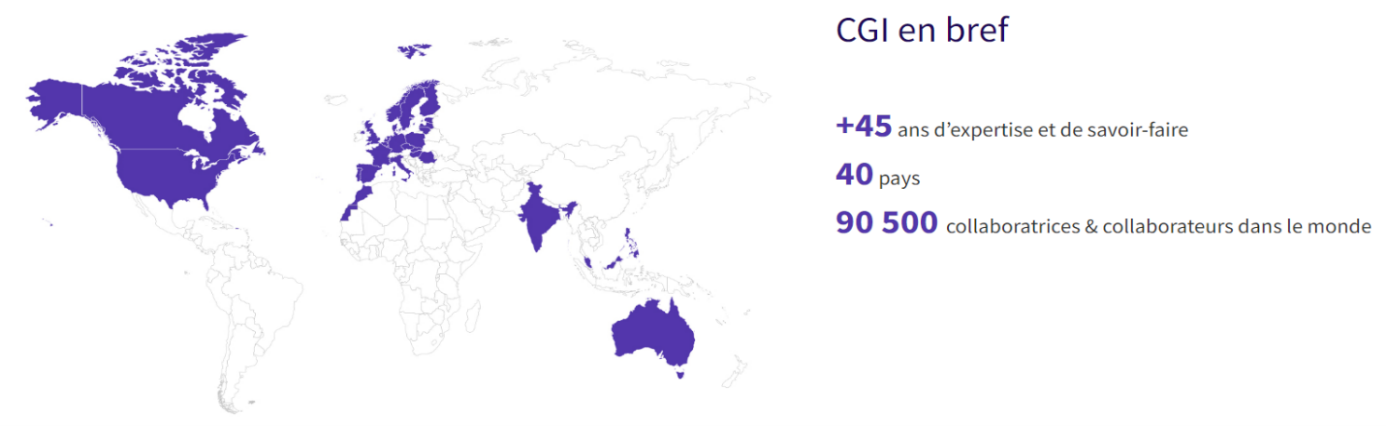
\includegraphics[width=0.8\linewidth]{imgs/entrprise_monde.png}
\caption{CGI dans le monde}
\label{fig:cgi_monde}
\end{figure}

\section{Secteurs d'activités}

CGI intervient dans une grande diversité de secteurs d'activité, offrant
ainsi à ses collaborateurs la possibilité de se spécialiser dans
différents domaines. Que ce soit dans la finance, l'énergie, les
télécommunications, l'industrie, la distribution, les transports ou
encore le secteur public, l'entreprise met à disposition de ses clients
une expertise ciblée, répondant à leurs besoins spécifiques.

Dans le secteur des services financiers, CGI accompagne les banques,
compagnies d'assurance et sociétés de gestion dans leur transformation
numérique, la gestion des risques, le respect des réglementations et
l'amélioration de l'expérience client.

Dans le domaine des télécommunications, elle fournit des solutions
innovantes aux opérateurs, fournisseurs de services numériques, médias
et entreprises de divertissement, en couvrant des aspects tels que la
gestion des réseaux, les services cloud, la cybersécurité et la
transformation digitale.

Concernant le secteur public, CGI collabore avec les administrations
nationales, régionales et locales pour développer des services
numériques visant à moderniser les services publics, renforcer la
sécurité informatique, optimiser la gestion des ressources et favoriser
l'innovation.

Dans le secteur de la santé, l'entreprise soutient les organismes de
soins, les hôpitaux et les entreprises pharmaceutiques à travers des
solutions digitales permettant d'améliorer la gestion des dossiers
médicaux, les processus cliniques et la recherche en santé.

En matière d'énergie, CGI intervient dans la gestion intelligente des
réseaux, la protection des infrastructures critiques, l'intégration des
énergies renouvelables et l'optimisation des ressources énergétiques.

Enfin, dans le commerce et la distribution, CGI accompagne les
entreprises dans leur digitalisation, en optimisant la chaîne
logistique, la gestion des stocks, l'expérience client multicanale et
l'exploitation des données.

Ces exemples témoignent de la capacité de CGI à s'adapter aux
spécificités de chaque secteur, en fournissant des solutions sur mesure.
Grâce à une connaissance approfondie des enjeux propres à chaque
domaine, l'entreprise se positionne comme un partenaire stratégique pour
les organisations, alliant flexibilité, expertise sectorielle et
innovation.

\section{Services de CGI}

\begin{figure}[H]
\centering
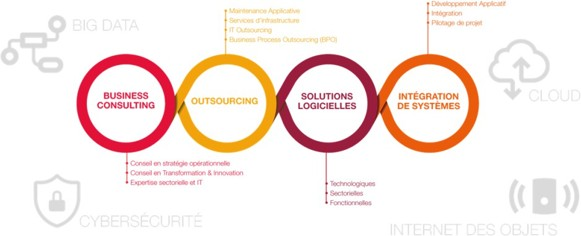
\includegraphics[width=0.8\linewidth]{imgs/service_cgi.jpg}
\caption{Services CGI}
\label{fig:services_cgi}
\end{figure}

CGI propose une large palette de services couvrant plusieurs domaines
d'activité et répondant aux besoins variés des organisations. Parmi les
principales prestations offertes, on peut citer :

\begin{itemize}
\item
  \textbf{Conseil en stratégie et en transformation numérique} : CGI
  accompagne les entreprises dans l'élaboration de leur vision
  numérique. Elle les aide à définir des plans de transformation adaptés
  à leurs objectifs et à piloter le changement de manière structurée.
\item
  \textbf{Intégration de systèmes} : l'entreprise intervient dans
  l'intégration de solutions technologiques au sein des infrastructures
  existantes, en veillant à assurer l'interopérabilité, la fluidité et
  l'efficacité des systèmes mis en place.
\item
  \textbf{Développement d'applications} : CGI conçoit et déploie des
  applications sur mesure, en s'appuyant sur les technologies les plus
  récentes et des méthodes de développement éprouvées, afin de répondre
  précisément aux exigences fonctionnelles des clients.
\item
  \textbf{Gestion de l'infrastructure et des opérations} : elle offre
  des services de supervision, de maintenance et de support technique
  pour garantir la disponibilité, la performance et la sécurité des
  environnements informatiques.
\item
  \textbf{Gestion des données} : CGI propose des solutions permettant de
  collecter, structurer, analyser et valoriser les données afin de
  soutenir la prise de décision et d'optimiser la performance des
  organisations.
\item
  \textbf{Cybersécurité} : l'entreprise déploie des dispositifs de
  protection avancés pour sécuriser les systèmes d'information, prévenir
  les menaces et réagir efficacement en cas d'incident.
\item
  \textbf{Optimisation des processus métiers} : enfin, CGI aide les
  entreprises à améliorer leur performance opérationnelle en modélisant,
  automatisant et optimisant leurs processus internes, dans une logique
  d'efficacité, de qualité et de satisfaction client.
\end{itemize}

\section{Partenaires de CGI}

CGI développe des partenariats stratégiques avec de grandes entreprises
technologiques reconnues à l'échelle mondiale. Parmi ses principaux
partenaires figurent notamment Microsoft, Oracle, SAP, Salesforce, IBM,
Amazon Web Services (AWS) et Google Cloud. Ces alliances permettent à
CGI d'accéder aux technologies les plus avancées, de renforcer sa
capacité d'innovation et de proposer à ses clients des solutions
intégrées et performantes.

En collaborant avec ces acteurs majeurs du secteur, CGI bénéficie d'une
expertise complémentaire et d'une portée accrue sur le marché
international. Par ailleurs, l'entreprise s'associe également avec des
partenaires spécialisés dans des domaines spécifiques tels que la
cybersécurité, l'intelligence artificielle, l'Internet des objets (IoT)
ou encore les technologies émergentes.

\begin{figure}[H]
\centering

\includegraphics[width=0.8\linewidth]{imgs/partenaire.jpg}
\caption{Partenaires de CGI}
\label{fig:partenaires_cgi}
\end{figure}

Cette approche fondée sur la collaboration et la complémentarité
technologique consolide la position de CGI en tant que partenaire
fiable, capable de relever des défis complexes et de proposer des
solutions innovantes, au service de la transformation et du
développement de ses clients.

\section{Clients de CGI}

CGI dispose d'un portefeuille de clients à l'échelle internationale,
composé majoritairement de grandes institutions issues de secteurs
variés. En mars 2015, les États-Unis représentaient la part la plus
importante de cette clientèle, avec 29 \% des contrats. Le Canada
occupait la deuxième position avec 15 \%, suivi de l'Europe, qui
constitue également une zone de présence significative pour
l'entreprise. Le reste du monde représentait environ 15 \% des
engagements contractuels de CGI.

Cette répartition témoigne de la forte implantation de CGI sur les
principaux marchés mondiaux, ainsi que de sa capacité à répondre aux
besoins d'organisations variées, tout en tenant compte des spécificités
locales.

Ci-dessous l'ensemble des clients clés de CGI.

\begin{figure}[H]
\centering
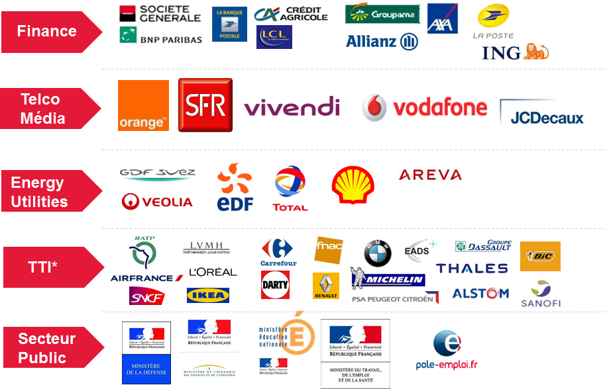
\includegraphics[width=0.8\linewidth]{imgs/clients_entreprise.png}
\caption{Les clients clés de CGI}
\label{fig:clients_cgi}
\end{figure}

\section{CGI Maroc}

\textbf{CGI Maroc} joue un rôle stratégique en tant que centre de
services reliant les marchés d'Amérique, d'Europe et d'Afrique. Depuis
son implantation en \textbf{2004}, l'entreprise accompagne les acteurs
majeurs de secteurs tels que l'énergie, la distribution, l'aéronautique
et la finance dans leurs projets de transformation numérique. Elle
mobilise plus de 1 300 professionnels répartis sur trois sites
(Casablanca, Rabat et Fès) et s'appuie sur une large gamme de
technologies, allant de la gestion des données aux systèmes
d'information complexes (CRM, ERP, NTIC, solutions héritées), afin de
répondre aux besoins spécifiques de ses clients internationaux.

Reconnue pour la qualité de ses prestations, \textbf{CGI} Maroc est
certifiée \textbf{ISO 9001} et \textbf{ISO 27001}, gages d'un engagement
fort en matière de qualité et de sécurité de l'information. Sa position
de leader dans le secteur des services informatiques au Maroc fait
d'elle un acteur clé du modèle Near-Shore, notamment dans l'espace
francophone.

Grâce à cette proximité géographique et culturelle avec l'Europe,
\textbf{CGI} peut établir des partenariats solides avec ses clients, en
leur apportant une expertise à la fois technologique et
organisationnelle. Elle accompagne aujourd'hui 35 clients actifs, dont
plusieurs grandes entreprises françaises, et pilote environ une
cinquantaine de projets numériques.

Par sa capacité à proposer des solutions innovantes et personnalisées,
\textbf{CGI} Maroc se positionne comme un partenaire fiable et
incontournable dans la conduite du changement et le développement
digital des organisations.

\begin{figure}[H]
\centering
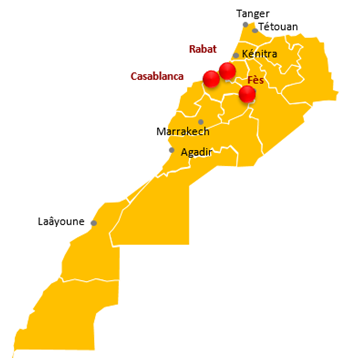
\includegraphics[width=0.8\linewidth]{imgs/entreprise_maroc.png}
\caption{Présence de CGI au Maroc}
\label{fig:presence_maroc}
\end{figure}

\section{Activités CGI Maroc}

\textbf{CGI Maroc} accompagne aujourd'hui plus de \textbf{45 clients}
répartis dans six grands secteurs d'activité, en leur proposant une
offre de services diversifiée et adaptée à leurs enjeux métiers.
L'entreprise met en œuvre son expertise à travers les prestations
suivantes :

\begin{itemize}
\item
  \textbf{Intégration de systèmes} : conception, développement et
  intégration de systèmes et d'applications visant à optimiser les
  processus opérationnels et à renforcer l'efficacité des organisations.
\item
  \textbf{Gestion des applications} : modernisation et restructuration
  des systèmes d'information pour soutenir les processus métier et
  atteindre les objectifs de performance définis.
\item
  \textbf{Gestion de l'infrastructure} : mise en place d'une
  architecture d'entreprise cohérente, couvrant à la fois le conseil
  stratégique, la planification et la mise en œuvre technique.
\item
  \textbf{Services de tests gérés} : élaboration de processus de test
  structurés et mise à disposition d'environnements adaptés, afin de
  garantir la fiabilité et la qualité des livrables.
\item
  \textbf{Externalisation des processus métiers (BPO)} : prise en charge
  de certaines fonctions ou activités de l'entreprise cliente par CGI,
  permettant ainsi une concentration accrue sur les missions
  stratégiques.
\item
  \textbf{Support technique et fonctionnel} : accompagnement
  personnalisé visant à maximiser les investissements technologiques des
  clients, à travers des actions de formation, de conseil continu et de
  support spécialisé.
\end{itemize}

\section{L'organigramme de CGI Maroc -- site de Fès}

Fort d'une expérience de plus de soixante ans, CGI s'impose comme un
acteur historique et une référence incontournable dans son domaine.
Cette position de leader repose avant tout sur la qualité de ses
ressources humaines : des femmes et des hommes hautement qualifiés,
engagés et porteurs de l'excellence opérationnelle.

Dans une démarche de croissance continue, l'entreprise a structuré son
organisation interne de manière à renforcer sa performance tout en
accroissant sa visibilité sur le marché. À travers une gestion
participative et la mise en place d'un fonctionnement transversal, CGI
valorise l'implication de ses collaborateurs dans les processus
décisionnels et le développement de leurs unités respectives.

Par ailleurs, CGI a renouvelé sa stratégie de recrutement, en cohérence
avec ses valeurs et sa culture d'entreprise. Cette orientation place le
capital humain au cœur du développement de l'organisation, favorisant
ainsi un environnement fondé sur la responsabilité, l'équité et la
transparence. Les effets positifs de cette approche se reflètent
clairement dans les résultats obtenus et la dynamique interne de
l'entreprise.

L'organigramme présenté ci-dessous illustre l'organisation interne de
\textbf{CGI Maroc -- site de Fès}, structure au sein de laquelle s'est
déroulé mon stage.

\begin{figure}[H]
\centering
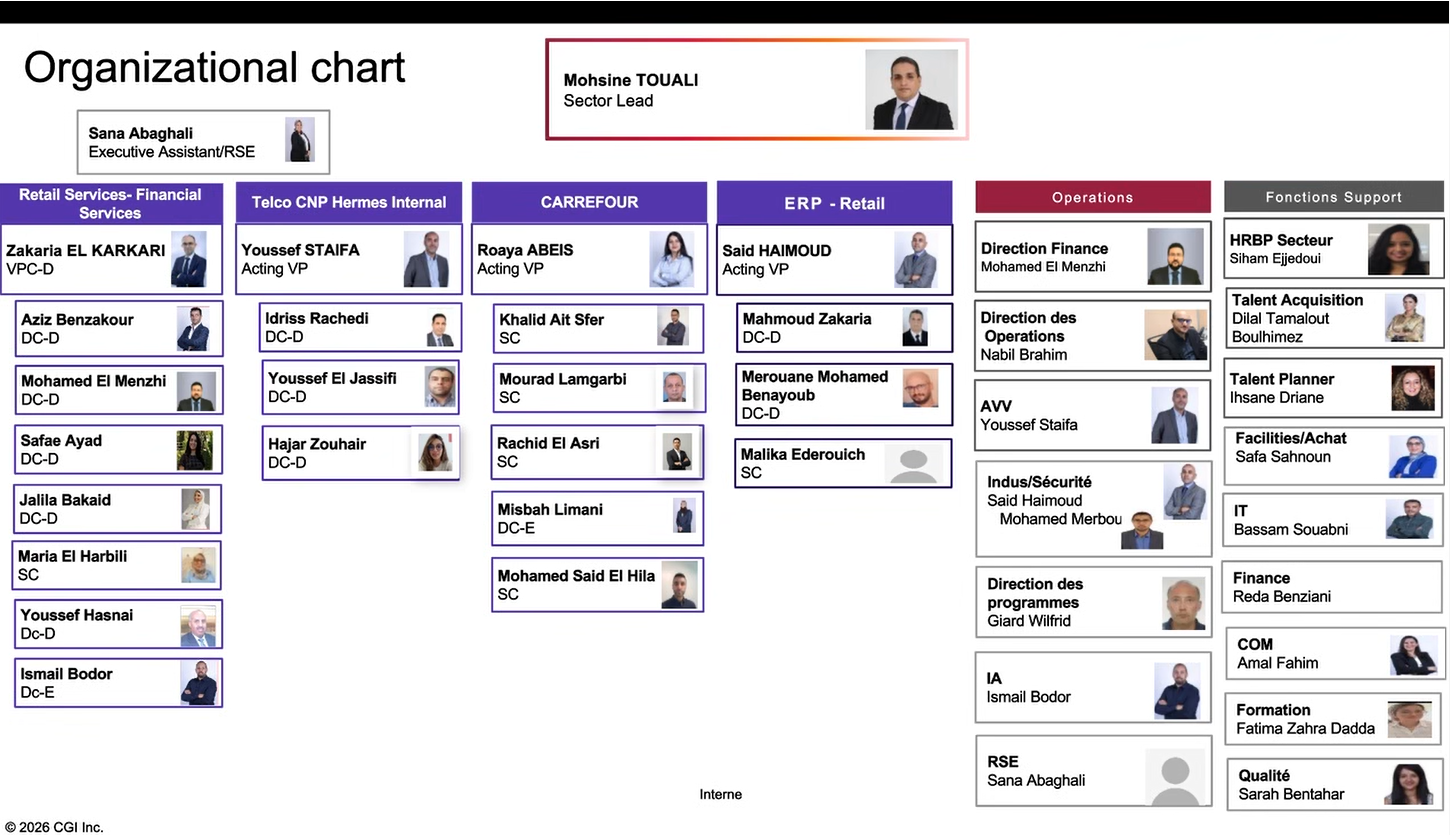
\includegraphics[width=0.8\linewidth]{imgs/organi1.png}
\caption{Organigramme de CGI Maroc -- site de Fès}
\label{fig:organigramme_fes}
\end{figure}

\newpage

% =========================================================================
% CHAPITRE 2 : INTRODUCTION ET PROBLEMATIQUE
% =========================================================================
\chapter{Introduction et Problématique}

\section{Contexte du Projet}
Dans le paysage technologique actuel, les bases de code grandissent plus vite que la
documentation qui les accompagne. Un développeur qui rejoint un projet, ou qui revient
sur un module qu'il n'a pas touché depuis plusieurs mois, doit reconstruire mentalement
la structure du système à partir du code source seul -- un exercice long et sujet à
erreur. Les outils existants qui automatisent cette tâche par l'IA générative
(résumés de fonctions, réponses à des questions sur un dépôt) reposent presque
systématiquement sur l'envoi du code source à une API cloud (OpenAI, Anthropic,
etc.), ce qui est inacceptable pour des bases de code propriétaires, sous contrat de
confidentialité, ou simplement sensibles.

C'est dans ce contexte qu'a été conçu et développé le projet présenté dans ce rapport :
\textbf{un outil local de génération automatique de documentation de code}. Il
transforme un dépôt de code source en un wiki de documentation navigable,
enrichi par l'IA, et interrogeable en langage naturel -- en exécutant
\textit{l'intégralité} du traitement (analyse statique, résumés, recherche
sémantique, réponses aux questions) sur la machine de l'utilisateur, sans qu'aucune
ligne de code, aucun résumé ni aucun embedding ne quitte jamais cette machine.

Le projet est structuré comme un pipeline modulaire de paquets Python, chacun avec
une responsabilité unique (scanner, analyseur syntaxique, graphe de dépendances,
moteur IA local, générateur de wiki, etc.), construit de manière incrémentale et
spécifiée, fonctionnalité par fonctionnalité, à travers une trentaine de
spécifications numérotées (\texttt{specs/001-\dots} à \texttt{specs/018-\dots}).

\section{La Problématique}
La conception d'un tel outil pose plusieurs défis majeurs auxquels ce projet tente de
répondre :
\begin{enumerate}
    \item \textbf{Confidentialité du code source} : comment générer une documentation
    assistée par IA sans jamais transmettre le code, ses résumés ou ses embeddings à
    un service tiers -- y compris de manière incidente, via un SDK cloud ou un
    repli silencieux en cas d'indisponibilité du service local ?
    \item \textbf{Documentation qui se périme} : une documentation rédigée
    manuellement diverge presque toujours du code au fil des modifications. Comment
    garantir qu'elle reste synchronisée avec le code, en continu, sans intervention
    humaine ?
    \item \textbf{Coût de la ré-analyse complète} : sur un dépôt volumineux déjà
    indexé, ré-analyser l'intégralité du code à chaque modification d'un seul fichier
    est prohibitif en temps de calcul. Comment ne retraiter que ce qui est réellement
    impacté par un changement, tout en garantissant un résultat final strictement
    identique à celui d'une ré-indexation complète ?
    \item \textbf{Traçabilité de l'IA générative} : un résumé de module ou une réponse
    de chat générés par un modèle de langage peuvent être plausibles sans être exacts
    (hallucination). Comment garantir que chaque affirmation générée soit
    rattachable, par une citation vérifiable, aux fichiers et symboles du code source
    qui la justifient ?
    \item \textbf{Hétérogénéité des langages} : un dépôt réel mélange souvent
    plusieurs langages (Python, JavaScript/TypeScript, Java, Go, Rust). Comment
    construire une seule chaîne d'analyse capable de produire un graphe de
    dépendances cohérent à travers ces langages, sans écrire un analyseur syntaxique
    différent pour chacun ?
\end{enumerate}

\section{Objectifs du Projet}
L'objectif principal est de concevoir, implémenter et valider un pipeline local
d'indexation, d'enrichissement par IA et de documentation de code, entièrement
auditable et sans dépendance réseau externe. La solution doit intégrer :
\begin{itemize}
    \item Une couche d'ingestion multi-langage (analyse syntaxique via
    \textbf{Tree-sitter}, extraction de symboles, imports et appels).
    \item Un \textbf{graphe de dépendances} et des \textbf{métadonnées persistées}
    (hash de contenu par fichier) permettant de savoir, à tout instant, ce qui a
    changé depuis la dernière analyse.
    \item Un accès à un \textbf{modèle de langage local} et à un \textbf{moteur
    d'embeddings local} (convention compatible Ollama, exposée uniquement sur
    \texttt{localhost}) pour générer des résumés de code et des vecteurs
    sémantiques.
    \item Un \textbf{wiki de documentation} généré automatiquement, navigable, avec
    des diagrammes de dépendances cliquables.
    \item Un \textbf{chat en langage naturel} (RAG) répondant aux questions sur le
    code, avec citations vérifiables vers les symboles et fichiers sources.
    \item Un \textbf{pipeline de ré-indexation incrémentale}, déclenché par la
    surveillance du dépôt en arrière-plan, dont le résultat final doit être identique
    à celui d'une ré-indexation complète.
\end{itemize}

\newpage

% =========================================================================
% CHAPITRE 3 : ARCHITECTURE TECHNIQUE ET UML
% =========================================================================
\chapter{Architecture de la Solution \& Modélisation}

\section{Architecture Globale du Système}
La solution est conçue comme un \textbf{pipeline local modulaire}, et non comme un
système distribué : chaque « service » (LLM local, moteur d'embeddings, serveur web)
s'exécute sur \texttt{127.0.0.1}, sur la machine même du développeur. Les paquets
Python communiquent entre eux par appel de fonction direct, en un seul processus --
il n'y a ni broker de messages, ni orchestrateur, ni frontière micro-service entre
les étapes. La figure \ref{fig:architecture} détaille l'organisation en cinq couches
du système et la boucle d'automatisation qui les maintient à jour.

\begin{figure}[H]
\centering
\resizebox{\textwidth}{!}{%
\begin{tikzpicture}[
    svc/.style   = {draw, rectangle, rounded corners=3pt,
                    minimum width=3.1cm, minimum height=1cm,
                    align=center, font=\scriptsize, drop shadow},
    ext/.style   = {draw, rectangle, rounded corners=3pt,
                    minimum width=3.1cm, minimum height=1cm,
                    align=center, fill=gray!10, draw=gray!70,
                    font=\scriptsize, drop shadow},
    arr/.style   = {-Latex, thick, draw=gray!70},
    dasharr/.style = {-Latex, thick, dashed, draw=purple!70},
    lbl/.style   = {font=\tiny, fill=white, inner sep=1pt},
]

    % ── Entrée externe ──
    \node[ext] (repo) at (0, 9) {D\'ep\^ot Git\\(lecture seule)};

    % ── Couche 1 : Ingestion \& Analyse (y = 9) ──
    \node[svc, fill=blue!10, draw=blue!60] (scan) at (4, 9) {repo\_scanner};
    \node[svc, fill=blue!10, draw=blue!60] (parse) at (8, 9) {parser\_engine\\(Tree-sitter)};
    \node[svc, fill=blue!10, draw=blue!60] (graph) at (12, 9) {dependency\_graph};
    \node[svc, fill=blue!10, draw=blue!60] (meta) at (17, 9) {repository\_metadata\\(hash de contenu)};

    % ── Couche 2 : Services IA locaux (y = 5.5) ──
    \node[svc, fill=orange!10, draw=orange!80] (llm) at (7.5, 5.5) {local\_llm};
    \node[svc, fill=orange!10, draw=orange!80] (emb) at (12.5, 5.5) {embedding\_engine};

    % ── Endpoint local, entre les deux (y = 3) ──
    \node[ext, fill=orange!8, draw=orange!70] (endpoint) at (10, 3) {Endpoint local\\Ollama-compatible\\(127.0.0.1:11434)};

    % ── Couche 3 : Dérivation de connaissance (y = 0) ──
    \node[svc, fill=teal!10, draw=teal!70] (summary) at (4, 0) {CodeSummaryPipeline};
    \node[svc, fill=teal!10, draw=teal!70] (vec) at (8, 0) {vector\_index};
    \node[svc, fill=teal!10, draw=teal!70] (chat) at (12, 0) {chat (RAG)};

    % ── Couche 4 : Présentation (y = -4) ──
    \node[svc, fill=green!10, draw=green!60!black] (doc) at (4, -4) {doc\_generator};
    \node[svc, fill=green!10, draw=green!60!black] (api) at (8.5, -4) {chat\_api\\(FastAPI, :127.0.0.1)};
    \node[svc, fill=green!10, draw=green!60!black] (ui) at (13, -4) {frontend\\(wiki-ui, React)};

    % ── Couche 5 : Automatisation (y = -8) ──
    \node[svc, fill=purple!10, draw=purple!70] (watch) at (4, -8) {repo\_watcher};
    \node[svc, fill=purple!10, draw=purple!70] (reindex) at (8.5, -8) {reindex\_pipeline};

    \node[ext] (reader) at (13, -8) {Membre d'\'equipe\\(navigateur)};

    % ── Flux d'indexation (gris) ──
    \draw[arr] (repo) -- (scan);
    \draw[arr] (scan) -- (parse);
    \draw[arr] (parse) -- (graph);
    \draw[arr] (graph) -- (meta);
    \draw[arr] (graph.south) -- ++(0,-2) -| node[lbl,pos=0.25,above]{contexte} (summary.north);
    \draw[arr] (meta.south) -- ++(0,-1.7) -| (summary.north east);
    \draw[arr] (summary.east) -- (vec.west);
    \draw[arr] (vec.east) -- (chat.west);
    \draw[arr] (summary.south) -- (doc.north);
    \draw[arr] (doc) -- (api);
    \draw[arr] (chat.south) -- ++(0,-1.3) -| (api.north east);
    \draw[arr] (api) -- (ui);
    \draw[arr] (ui) -- (reader);

    % ── Appels IA locaux (orange) ──
    \draw[arr, draw=orange!80] (summary.north) -- ++(0,1.4) -| node[lbl,pos=0.3,above]{generate()} (llm.south);
    \draw[arr, draw=orange!80] (vec.north) -- ++(0,1.6) -| node[lbl,pos=0.3,above]{embed()} (emb.south);
    \draw[arr, draw=orange!80] (chat.north) -- ++(0,1.8) -| (llm.south east);
    \draw[arr, draw=orange!80] (llm) -- (endpoint);
    \draw[arr, draw=orange!80] (emb) -- (endpoint);

    % ── Boucle d'automatisation (violet, pointillé) ──
    \draw[dasharr] (repo.south) |- node[lbl, pos=0.05, left]{surveille} (watch.west);
    \draw[dasharr] (watch) -- node[lbl, above]{lot de fichiers modifi\'es} (reindex);
    \draw[dasharr] (reindex.east) -| node[lbl, pos=0.85, above]{mise \`a jour cibl\'ee} (meta.south);
    \draw[dasharr] (reindex.north) -- ++(0,1.5) -- ++(-9.5,0) -- ++(0,6) -- node[lbl,pos=0.9,above]{r\'eg\'en\`ere} (summary.west);

    % ── Légende ──
    \node[anchor=north west, font=\tiny, text=gray] at (-1.5, -10.3) {%
        \textcolor{gray!70}{\rule{0.6cm}{2pt}} Flux d'indexation \quad
        \textcolor{orange!80}{\rule{0.6cm}{2pt}} Appels IA locaux (localhost) \quad
        \textcolor{purple!70}{\rule[0.4ex]{0.6cm}{1pt}} Boucle de r\'e-indexation incr\'ementale
    };

\end{tikzpicture}%
}% end resizebox
\caption{Architecture en cinq couches du système et boucle d'automatisation locale}
\label{fig:architecture}
\end{figure}

Par souci de lisibilité, le schéma ne représente pas explicitement la relation entre
\texttt{dependency\_graph} et \texttt{doc\_generator} (les diagrammes de dépendances
intégrés aux pages générées) : \texttt{doc\_generator} interroge directement le graphe
au moment de la génération, comme le montre le diagramme de classes (Figure
\ref{fig:uml_classes}).

\section{Isolation locale et stockage}
N'étant pas un système distribué, l'architecture n'a pas besoin de segmentation
réseau par conteneurs : l'isolation repose sur deux principes structurants,
directement issus de la constitution du projet.

\begin{itemize}
    \item \textbf{Aucune exposition réseau par défaut} : le seul processus de longue
    durée du système, \texttt{chat\_api} (FastAPI/Uvicorn), se lie à
    \texttt{127.0.0.1} par défaut -- aucune interface n'est accessible depuis le
    réseau sans action explicite de l'utilisateur.
    \item \textbf{Un fichier SQLite par composant} : \texttt{repository\_metadata},
    \texttt{dependency\_graph}, \texttt{vector\_index} et \texttt{doc\_generator}
    possèdent chacun leur propre fichier SQLite, écrit exclusivement par le
    composant qui le possède. Aucun serveur de base de données externe n'est
    utilisé -- le stockage embarqué (SQLite) est la seule forme de persistance
    autorisée.
\end{itemize}

\section{Modélisation UML : Diagramme de Séquence -- Ré-indexation Incrémentale}
La fonctionnalité la plus critique du système est sa capacité à mettre à jour la
documentation d'un dépôt déjà indexé sans jamais relancer une analyse complète. La
figure \ref{fig:uml_sequence} détaille l'enchaînement des appels lorsqu'un
développeur modifie un fichier : la surveillance du dépôt (\texttt{repo\_watcher})
déclenche le pipeline de ré-indexation (\texttt{reindex\_pipeline}), qui confirme le
changement via le hash de contenu stocké en base avant tout retraitement coûteux, ne
régénère que les symboles réellement impactés, et met à jour uniquement les
embeddings et pages de documentation concernés.

\begin{figure}[H]
\centering
\resizebox{\textwidth}{!}{%
\begin{tikzpicture}[
    actor/.style={draw, circle, fill=yellow!20, minimum size=0.6cm, font=\small},
    obj/.style={draw, rectangle, fill=blue!10, minimum width=2.6cm, minimum height=0.9cm, font=\scriptsize, align=center},
    lifeline/.style={draw, dashed, thick, gray!80},
    active/.style={draw, fill=blue!5, minimum width=0.3cm}
]

    % Acteurs et Lifelines
    \node[actor] (dev) at (0, 0) {Dev};
    \node[obj] (watch) at (3.5, 0) {repo\_watcher};
    \node[obj] (reindex) at (7.5, 0) {reindex\_pipeline};
    \node[obj] (meta) at (11.5, 0) {dependency\_graph\\+ repository\_metadata};
    \node[obj] (ai) at (15.5, 0) {CodeSummaryPipeline\\+ vector\_index};
    \node[obj] (doc) at (19, 0) {doc\_generator};

    % Lifeline Paths
    \draw[lifeline] (dev) -- (0, -9);
    \draw[lifeline] (watch) -- (3.5, -9);
    \draw[lifeline] (reindex) -- (7.5, -9);
    \draw[lifeline] (meta) -- (11.5, -9);
    \draw[lifeline] (ai) -- (15.5, -9);
    \draw[lifeline] (doc) -- (19, -9);

    % Activation boxes
    \node[active, minimum height=8cm] (dev_act) at (0, -4.5) {};
    \node[active, minimum height=7cm] (watch_act) at (3.5, -4) {};
    \node[active, minimum height=6cm] (reindex_act) at (7.5, -3.5) {};
    \node[active, minimum height=2.2cm] (meta_act) at (11.5, -3) {};
    \node[active, minimum height=2.2cm] (ai_act) at (15.5, -5.3) {};
    \node[active, minimum height=1.2cm] (doc_act) at (19, -7.6) {};

    % Messages
    \draw[-Latex, thick] (0, -1) -- node[above, font=\tiny] {1. modifie un fichier} (3.5, -1);
    \node[align=left, anchor=west, font=\tiny\ttfamily] at (3.7, -1.5) {D\'ebounce, attend\\la stabilisation};

    \draw[-Latex, thick] (3.5, -2.2) -- node[above, font=\tiny, align=center] {2. lot de fichiers modifi\'es} (7.5, -2.2);

    \draw[-Latex, thick] (7.5, -3) -- node[above, font=\tiny] {3. hash de contenu ?} (11.5, -3);
    \draw[Latex-, thick, dashed] (7.5, -3.6) -- node[below, font=\tiny] {4. chang\'e / inchang\'e} (11.5, -3.6);

    \node[align=left, anchor=west, font=\tiny\ttfamily, color=red!70] at (7.7, -4.2) {Si inchang\'e :\\arr\^ete ici (co\^ut nul)};

    \draw[-Latex, thick] (7.5, -5) -- node[above, font=\tiny, align=center] {5. re-parse + met \`a jour\\le graphe / m\'etadonn\'ees} (11.5, -5);

    \draw[-Latex, thick] (7.5, -5.7) -- node[above, font=\tiny, align=center] {6. r\'eg\'en\`ere r\'esum\'e + embedding\\des symboles impact\'es} (15.5, -5.7);

    \draw[Latex-, thick, dashed] (7.5, -6.4) -- node[below, font=\tiny] {7. symboles r\'eg\'en\'er\'es} (15.5, -6.4);

    \draw[-Latex, thick] (7.5, -7.6) -- node[above, font=\tiny, align=center] {8. r\'eg\'en\`ere uniquement\\les pages impact\'ees} (19, -7.6);

    \node[align=left, anchor=west, font=\tiny\ttfamily, color=teal] at (7.7, -8.5) {Le r\'esultat final est identique\\\`a une r\'e-indexation compl\`ete};

\end{tikzpicture}%
}
\caption{Diagramme de séquence UML : ré-indexation incrémentale déclenchée par le watcher}
\label{fig:uml_sequence}
\end{figure}

\newpage

\section{Modélisation UML : Diagramme de Classes}
Le diagramme de classes (Figure \ref{fig:uml_classes}) détaille les classes clés
impliquées dans le pipeline de ré-indexation incrémentale et leurs collaborations
avec les couches d'analyse et de dérivation de connaissance.

\begin{figure}[H]
\centering
\resizebox{\textwidth}{!}{%
\begin{tikzpicture}[
    class/.style={draw, rectangle, rounded corners=2pt, fill=blue!5,
                  draw=blue!50!black, thick, minimum width=3.8cm,
                  align=left, font=\scriptsize},
    arrow/.style={-Latex, thick, draw=blue!50!black},
    aggr/.style={-{Diamond[open]}, thick, draw=blue!50!black}
]

    % ── Colonne 1 : orchestration (x=0) ──
    \node[class] (Reindex) at (0, 6) {
        \textbf{IncrementalReindexPipeline} \\
        \rule{3.5cm}{0.4pt} \\
        \\
        \rule{3.5cm}{0.4pt} \\
        + run(batch) : ReindexOutcome
    };

    \node[class] (Summary) at (0, 1) {
        \textbf{CodeSummaryPipeline} \\
        \rule{3.5cm}{0.4pt} \\
        \\
        \rule{3.5cm}{0.4pt} \\
        + summarizeRepository(root,\\
        \phantom{+ }incremental, changed\_paths)
    };

    \node[class] (MetaStore) at (0, -4) {
        \textbf{RepositoryMetadataStore} \\
        \rule{3.5cm}{0.4pt} \\
        \\
        \rule{3.5cm}{0.4pt} \\
        + store\_inventory(...) \\
        + has\_file\_changed(...) : bool \\
        + delete\_source\_file(...)
    };

    % ── Colonne 2 : données persistées (x=7) ──
    \node[class] (Graph) at (7, 4) {
        \textbf{DependencyGraph} \\
        \rule{3.5cm}{0.4pt} \\
        - nodes : dict[str, Node] \\
        \rule{3.5cm}{0.4pt} \\
        + ingest\_inventory(inv) \\
        + remove\_source\_file(f) \\
        + dependents(focus) : list
    };

    \node[class] (Bundle) at (7, -2) {
        \textbf{RepositoryBundle} \\
        \rule{3.5cm}{0.4pt} \\
        - repository : Repository \\
        - files : tuple[SourceFileBundle] \\
        \rule{3.5cm}{0.4pt}
    };

    % ── Colonne 3 : dérivation / présentation (x=14) ──
    \node[class] (Vector) at (14, 6) {
        \textbf{VectorIndex} \\
        \rule{3.5cm}{0.4pt} \\
        \\
        \rule{3.5cm}{0.4pt} \\
        + reindexFile(path, chunks) \\
        + removeChunksForFile(path) \\
        + search(query, k) : list
    };

    \node[class] (ChatSession) at (14, 1.5) {
        \textbf{ChatSession} \\
        \rule{3.5cm}{0.4pt} \\
        - messages : list[ChatMessage] \\
        \rule{3.5cm}{0.4pt} \\
        + ask(question) : ChatMessage
    };

    \node[class] (DocGen) at (14, -3.5) {
        \textbf{DocGenerator} \\
        \rule{3.5cm}{0.4pt} \\
        \\
        \rule{3.5cm}{0.4pt} \\
        + generateRepositoryDocumentation(\\
        \phantom{+ }root, incremental, changedPaths)
    };

    % ── Colonne 4 : sortie (x=21) ──
    \node[class] (Outcome) at (21, 6) {
        \textbf{ReindexOutcome} \\
        \rule{3.5cm}{0.4pt} \\
        - reprocessedPaths : tuple[str] \\
        - regeneratedSymbolIds : tuple[str] \\
        - failedPaths : tuple[str] \\
        \rule{3.5cm}{0.4pt}
    };

    \node[class] (DocSet) at (21, -3.5) {
        \textbf{DocumentationSet} \\
        \rule{3.5cm}{0.4pt} \\
        - pages : tuple[DocPage] \\
        \rule{3.5cm}{0.4pt}
    };

    % ── Associations (connexions nœud-à-nœud : TikZ ancre automatiquement
    %    sur le bord de chaque boîte, la ligne ne traverse donc jamais son
    %    intérieur, quel que soit l'angle) ──
    \draw[arrow] (Reindex) -- node[left, font=\tiny]{orchestre} (Summary);
    \draw[arrow] (Summary) -- (MetaStore);
    \draw[arrow] (Reindex) -- node[above, font=\tiny, pos=0.35]{maj cibl\'ee} (Graph);
    \draw[arrow] (MetaStore) -- (Bundle);
    \draw[arrow] (Summary) -- node[above, font=\tiny, pos=0.6]{dependents()} (Graph);
    \draw[arrow] (Reindex) -- node[above, font=\tiny]{maj cibl\'ee} (Vector);
    \draw[arrow] (Vector) -- (ChatSession);
    \draw[arrow] (Reindex) -- node[above, font=\tiny, pos=0.75]{maj cibl\'ee} (DocGen);
    \draw[aggr]  (DocGen) -- (DocSet);
    \draw[arrow] (Reindex.north) -- ++(0,1.0) -| (Outcome.north);

\end{tikzpicture}%
}% end resizebox
\caption{Diagramme de classes UML des composants impliqués dans le pipeline d'indexation}
\label{fig:uml_classes}
\end{figure}

\newpage

\section{Modélisation UML : Diagramme de Cas d'Utilisation}
Le diagramme de cas d'utilisation (Figure \ref{fig:uml_usecases}) définit les acteurs
du système -- humains et automatisés -- et leurs interactions avec les composants
logiciels.

\begin{figure}[H]
\centering
\resizebox{\textwidth}{!}{%
\begin{tikzpicture}[
    usecase/.style={draw, ellipse, fill=blue!5, draw=blue!50!black, thick, minimum width=3.8cm, minimum height=1.2cm, align=center, font=\scriptsize, inner sep=2pt},
    arrow/.style={-Latex, thick, draw=blue!50!black},
    extend/.style={-Latex, dashed, thick, draw=blue!50!black},
    actor_label/.style={font=\scriptsize\bfseries},
    actor/.style={thick}
]

    % System Boundary Box (dessinée en premier, sous tout le reste)
    \node[draw, gray, thick, fill=gray!3, rounded corners=5pt,
          minimum width=15cm, minimum height=17cm] (boundary) at (8.5, 0) {};
    \node[font=\scriptsize\bfseries\itshape] at (8.5, 8.9) {Outil local de documentation de code};

    % ── Cas d'usage : cha\^ine principale (colonne x=5) ──
    \node[usecase] (uc1) at (5, 7)    {Indexer un d\'ep\^ot\\(scan, parse, analyse)};
    \node[usecase] (uc2) at (5, 4.7)  {G\'en\'erer les r\'esum\'es\\de symboles (LLM local)};
    \node[usecase] (uc3) at (5, 2.4)  {Construire l'index\\vectoriel s\'emantique};
    \node[usecase] (uc4) at (5, 0.1)  {G\'en\'erer le wiki\\de documentation};
    \node[usecase] (uc5) at (5, -2.2) {Parcourir / rechercher\\dans la documentation};
    \node[usecase] (uc6) at (5, -4.5) {Poser une question\\(chat RAG, cit\'e)};
    \node[usecase] (uc7) at (5, -6.8) {Surveiller le d\'ep\^ot\\et r\'e-indexer};

    % ── Cas d'usage transversal (colonne de droite) ──
    \node[usecase, minimum width=4.6cm] (uc8) at (12.5, -1.2) {\'Echouer clairement plut\^ot\\que basculer vers le cloud};

    % ── Op\'erateur (gauche, haut) ──
    \draw[actor] (-0.7,7.3) circle (0.15);
    \draw[actor] (-0.7,7.15) -- (-0.7,6.65);
    \draw[actor] (-0.9,6.95) -- (-0.5,6.95);
    \draw[actor] (-0.7,6.65) -- (-0.9,6.3);
    \draw[actor] (-0.7,6.65) -- (-0.5,6.3);
    \node[actor_label] at (-0.7,6.0) {Op\'erateur};

    % ── Membre d'\'equipe (gauche, milieu) ──
    \draw[actor] (-0.7,-3.05) circle (0.15);
    \draw[actor] (-0.7,-3.2) -- (-0.7,-3.7);
    \draw[actor] (-0.9,-3.4) -- (-0.5,-3.4);
    \draw[actor] (-0.7,-3.7) -- (-0.9,-4.05);
    \draw[actor] (-0.7,-3.7) -- (-0.5,-4.05);
    \node[actor_label, align=center] at (-0.7,-4.4) {Membre\\d'\'equipe};

    % ── D\'eveloppeur (droite, haut) ──
    \draw[actor] (18,7.3) circle (0.15);
    \draw[actor] (18,7.15) -- (18,6.65);
    \draw[actor] (17.8,6.95) -- (18.2,6.95);
    \draw[actor] (18,6.65) -- (17.8,6.3);
    \draw[actor] (18,6.65) -- (18.2,6.3);
    \node[actor_label] at (18,6.0) {D\'eveloppeur};

    % ── repo\_watcher (droite, bas -- automatisation) ──
    \node[draw, rectangle, rounded corners=2pt, fill=purple!8, draw=purple!60,
          font=\scriptsize, align=center] (watcher) at (18, -6.8) {repo\_watcher\\(automatisation)};

    % ── Liens acteurs -> cas d'usage (auto-ancr\'es sur le bord des formes) ──
    \draw[arrow] (-0.5,6.95) -- (uc1);
    \draw[arrow] (-0.5,-3.4) -- (uc5);
    \draw[arrow] (-0.5,-3.4) -- (uc6);
    \draw[arrow] (18,6.3) -- (watcher);
    \draw[arrow] (watcher) -- (uc7);

    % ── Inclusions (cha\^ine verticale, colonnes altern\'ees pour la lisibilit\'e) ──
    \draw[extend] (uc1) -- node[right, font=\tiny\ttfamily] {<<include>>} (uc2);
    \draw[extend] (uc2) -- node[right, font=\tiny\ttfamily] {<<include>>} (uc3);
    \draw[extend] (uc3) -- node[right, font=\tiny\ttfamily] {<<include>>} (uc4);

    % ── uc7 <<include>> uc1 : contourne la cha\^ine par la gauche, \`a
    %    l'int\'erieur de la fronti\`ere syst\`eme, pour ne traverser aucune
    %    ellipse interm\'ediaire ──
    \draw[extend] (uc7.west) -- ++(-1.3,0) node[pos=0.5, below, font=\tiny\ttfamily] {<<include>>}
        -- ++(0,13.8) -- (uc1.west);

    % ── Extensions vers le cas d'\'echec ──
    \draw[extend] (uc2) -- node[above, font=\tiny\ttfamily, sloped] {<<extend>>} (uc8);
    \draw[extend] (uc6) -- node[below, font=\tiny\ttfamily, sloped] {<<extend>>} (uc8);

\end{tikzpicture}%
}
\caption{Diagramme de cas d'utilisation UML décrivant les acteurs et cas d'usage principaux}
\label{fig:uml_usecases}
\end{figure}

\newpage

% =========================================================================
% CHAPITRE 4 : LA STACK TECHNIQUE DETAILLEE ET RAISONNEE
% =========================================================================
\chapter{La Stack Technique Détaillée et Raisonnée}

L'évaluation et la justification des choix technologiques reposent sur trois
contraintes structurantes imposées par la constitution du projet : aucune
infrastructure lourde (pas de serveur de base de données, pas de broker), aucune
dépendance à un service cloud, et une empreinte minimale pour rester facile à
auditer et à faire fonctionner hors ligne.

\section{Tableau Comparatif et Décisions d'Architecture}
Le tableau \ref{tab:stack} résume l'analyse décisionnelle de la stack technique.

\begin{table}[H]
\centering
\small
\begin{tabular}{p{3.2cm}p{5.5cm}p{5.5cm}}
\toprule
\textbf{Composant} & \textbf{Technologie Retenue} & \textbf{Justification \& Alternative Rejetée} \\
\midrule
Analyse multi-langage & \textbf{Tree-sitter} + \texttt{ast} (Python) & \textit{Seul moyen réaliste d'obtenir un AST réel et tolérant aux erreurs sur six langages sans écrire six analyseurs.} Alternative rejetée : un analyseur dédié par langage (coût prohibitif). \\
\midrule
Graphe de dépendances & \textbf{Structure interne dédiée} (\texttt{dependency\_graph}) & \textit{Les besoins de requête sont étroits} (\texttt{dependents()}, \texttt{exportDiagram()}). Alternative rejetée : \texttt{networkx} (bibliothèque généraliste, complexité superflue). \\
\midrule
Persistance locale & \textbf{SQLite} (\texttt{sqlite3} standard) & \textit{Stockage embarqué, sans processus serveur} -- exigence directe de la constitution (§2.6). Alternative rejetée : PostgreSQL/MySQL (nécessite un serveur externe). \\
\midrule
Accès IA locale (LLM \& embeddings) & \textbf{HTTP brut} (\texttt{urllib}) vers un endpoint compatible \textbf{Ollama} & \textit{Aucune dépendance SDK pour deux appels JSON} ; l'URL est validée comme strictement locale au niveau du code. Alternative rejetée : SDK cloud propriétaire. \\
\midrule
Rendu de documentation & \textbf{Jinja2 + Python-Markdown} + \textbf{mermaid.js} vendored & \textit{Le wiki généré doit s'afficher intégralement hors ligne.} Alternative rejetée : \texttt{mermaid.js} via CDN (violerait le zéro exposition réseau). \\
\midrule
Serveur web / API & \textbf{FastAPI + Uvicorn}, lié à \texttt{127.0.0.1} & \textit{Modèles de requête/réponse typés (Pydantic)}, liaison loopback par défaut. Alternative rejetée : exposition sur \texttt{0.0.0.0} par défaut. \\
\bottomrule
\end{tabular}
\\ \vspace{0.2cm}
\caption{Analyse raisonnée des choix technologiques}
\label{tab:stack}
\end{table}

\section{Justification Technique des Choix Clés}

\subsection{Confidentialité imposée au niveau du code, pas seulement de la politique}
Le principe « aucune ligne de code ne quitte la machine » n'est pas qu'une
recommandation documentée : il est vérifié programmatiquement. Chaque endpoint
IA local (LLM comme embeddings) passe par une fonction de normalisation qui rejette
toute URL dont l'hôte n'est pas \texttt{localhost}, \texttt{127.0.0.1} ou
\texttt{::1}, avant même la première requête HTTP.

\begin{lstlisting}[language=python, caption={Validation stricte de l'endpoint local (\texttt{src/local\_llm/models.py})}]
def normalize_endpoint_url(endpoint_url: str) -> str:
    parsed = urlparse(endpoint_url)
    if parsed.scheme not in {"http", "https"}:
        raise ValueError("endpointUrl must use http or https")
    if not parsed.hostname:
        raise ValueError("endpointUrl must include a hostname")
    if parsed.hostname not in {"localhost", "127.0.0.1", "::1"}:
        raise ValueError("endpointUrl must point to a local host")
    if parsed.path not in {"", "/"}:
        raise ValueError("endpointUrl must not include a path")
    return endpoint_url.rstrip("/")
\end{lstlisting}

Il devient ainsi structurellement impossible de pointer, même par erreur de
configuration, le pipeline de résumé ou d'embeddings vers une API cloud.

\subsection{Un fichier SQLite par composant, pas une base partagée}
\begin{sloppypar}
Plutôt qu'un schéma unique partagé, chaque composant (\path{repository_metadata},
\path{dependency_graph}, \path{vector_index}, \path{doc_generator}) possède
son propre fichier SQLite et en est le seul écrivain. Ce choix accepte une petite
duplication de code de connexion en échange d'une frontière de responsabilité
simple : aucun composant n'a besoin de comprendre le schéma d'un autre, et une
migration ne touche jamais qu'un seul fichier.
\end{sloppypar}

\subsection{Tree-sitter pour l'analyse multi-langage}
Tree-sitter est utilisé pour produire un AST réel, incrémental et tolérant aux
erreurs, à travers six langages (Python, JavaScript, TypeScript, Java, Go, Rust),
avec un module dédié par grammaire
(\texttt{tree-sitter-python}, \texttt{-javascript}, \texttt{-typescript},
\texttt{-java}, \texttt{-go}, \texttt{-rust}). Pour les fichiers \texttt{.py}, le
module \texttt{ast} natif de Python est utilisé comme voie rapide dédiée. Le
caractère tolérant aux erreurs de Tree-sitter est essentiel : un fichier contenant
une erreur de syntaxe continue de produire un arbre exploitable, ce qui permet au
pipeline de signaler l'échec sur ce fichier précis tout en poursuivant l'analyse du
reste du dépôt.

\newpage

% =========================================================================
% CHAPITRE 5 : RESILIENCE, CONFIDENTIALITE ET QUALITE
% =========================================================================
\chapter{Résilience, Confidentialité et Qualité}

Un outil qui analyse du code source pour le compte d'un développeur doit se
comporter de manière prévisible même dans les cas dégradés : service IA local
indisponible, fichier au contenu invalide, dépôt volumineux modifié en rafale. Ce
chapitre détaille les mécanismes de résilience mis en œuvre et la manière dont ils
ont été validés.

\section{Aucun repli silencieux vers un service cloud}
\begin{sloppypar}
Si le LLM local ou le moteur d'embeddings est indisponible, chaque composant
appelant échoue explicitement -- via \path{LocalLLMUnavailableError} côté
pipeline de résumé, ou \path{ServiceUnavailableError} côté \path{local_llm} et
\path{embedding_engine} -- plutôt que de basculer, même temporairement, vers un
service distant. Le pipeline de résumé (\texttt{CodeSummaryPipeline}) capture cette
exception spécifiquement, afin de continuer à traiter les autres flux (embeddings,
génération de documentation) au lieu de faire échouer l'intégralité d'une
ré-indexation à cause d'un seul service temporairement arrêté.
\end{sloppypar}

\section{Le dépôt analysé reste en lecture seule}
Aucun composant du système n'écrit jamais dans le dépôt qu'il analyse. Toute
écriture -- métadonnées, graphe, embeddings, pages de documentation générées -- est
dirigée vers un emplacement de stockage séparé, propre à l'outil. Cette contrainte,
inscrite dans la constitution du projet (§2.7), garantit que l'exécution de l'outil
sur un dépôt de production ne peut jamais en modifier le contenu, même en cas
d'erreur interne.

\section{Tolérance aux erreurs de parsing}
Grâce au caractère tolérant aux erreurs de Tree-sitter, un fichier syntaxiquement
invalide n'interrompt jamais le traitement d'un lot : son échec est capturé,
consigné (\texttt{failedPaths} dans le résultat de ré-indexation), et le reste du
lot continue d'être traité normalement.

\section{Étude de cas : la ré-indexation incrémentale doit être équivalente à une ré-indexation complète}
Le critère de succès le plus exigeant du pipeline de ré-indexation incrémentale
(spécification 018) est un critère d'\emph{équivalence} : le résultat obtenu après
la modification d'un seul fichier doit être strictement identique à celui obtenu en
ré-analysant l'intégralité du dépôt. Ce critère a directement révélé, pendant le
développement, un cas limite non trivial : les identifiants de nœuds du graphe de
dépendances sont dérivés du hash de contenu d'un symbole -- une mise à jour
incrémentale ne modifie donc pas un nœud existant, elle le \emph{remplace}. Or ce
remplacement supprimait silencieusement l'arête entrante d'un appelant externe
resté inchangé (et donc non retraité dans le même lot), cassant l'analyse d'impact
(\texttt{dependents()}) dont dépend toute la garantie « ne régénérer que ce qui est
directement impacté ».

Le correctif consiste à capturer les arêtes entrantes externes d'un symbole avant
son remplacement, puis à les relier par nom au nouveau nœud une fois celui-ci créé
(\path{_capture_external_incoming_edges} / \path{_relink_external_edges}
dans \path{reindex_pipeline/graph_sync.py}). Ce cas n'a été détecté que grâce à
un test d'intégration comparant explicitement, sur le même dépôt d'exemple, le
résultat d'une mise à jour incrémentale et celui d'une ré-indexation complète --
illustrant la valeur d'une validation par équivalence plutôt qu'une simple
validation « ça ne plante pas ».

\section{Validation par la suite de tests automatisés}
Le projet suit un seul et même schéma de test pour chacun de ses paquets --
\texttt{tests/unit/}, \texttt{tests/integration/}, \texttt{tests/contract/} -- ce
qui a permis, lors du développement de la spécification 018, de valider à la fois
le comportement isolé de chaque fonction (tests unitaires), le comportement de bout
en bout du pipeline sur un dépôt d'exemple multi-fichiers (tests d'intégration), et
la stabilité de l'interface publique exposée aux autres composants (tests de
contrat). L'ensemble de la suite -- plus de 145 tests -- passe, à l'exception de
trois tests préexistants, sans rapport avec cette fonctionnalité, en échec à cause
d'une incompatibilité de version de grammaire Tree-sitter.

\newpage

% =========================================================================
% CHAPITRE 6 : PIPELINE IA LOCALE
% =========================================================================
\chapter{Pipeline IA Locale : Résumés, Embeddings et Chat RAG}

Ce chapitre détaille la couche de dérivation de connaissance du système : comment
le code analysé est transformé en résumés lisibles, en un index recherchable par le
sens, et en réponses de chat justifiées.

\section{Génération de résumés contextualisés}
Pour chaque module et fonction publique, \texttt{CodeSummaryPipeline} construit un
prompt combinant le code source du symbole, ses imports, et ses appelants directs
(obtenus via \texttt{DependencyGraph.dependents()}), puis interroge le LLM local
pour produire un résumé en langage naturel. Lors d'une ré-indexation, seuls les
symboles dont le résumé dépend directement d'un fichier modifié sont régénérés --
jamais l'ensemble du dépôt.

\section{Index vectoriel et recherche sémantique}
Le moteur d'embeddings local transforme chaque fragment de code pertinent en un
vecteur, stocké par \texttt{vector\_index} aux côtés de l'identifiant du symbole
d'origine. Cela permet de retrouver du code par le sens de la requête plutôt que par
la seule correspondance de mots-clés -- par exemple, une recherche « où gère-t-on
l'authentification de l'utilisateur ? » peut retrouver une fonction nommée
\texttt{verify\_session} même si aucun de ces mots-clés n'apparaît littéralement dans
la requête.

\section{Chat RAG avec citations vérifiables}
Le chat répond à une question en récupérant d'abord les fragments de code les plus
pertinents via \texttt{vector\_index.search()}, puis en demandant au LLM local de
répondre \emph{en s'appuyant explicitement} sur ces fragments. Chaque message de
réponse conserve la liste des identifiants de symboles cités
(\texttt{citedSymbolIds}), ce qui permet à l'interface de wiki d'afficher des liens
cliquables vers les fichiers et symboles exacts qui justifient la réponse --
conformément au principe de traçabilité de la constitution (§2.4).

\begin{lstlisting}[caption={Structure simplifiée d'un message de réponse du chat, avec citations}]
{
  "role": "assistant",
  "content": "Confirme le changement via le hash de contenu stocke.",
  "citedSymbolIds": [
    "reindex_pipeline.classification.confirm_change",
    "repository_metadata.store.has_file_changed"
  ]
}
\end{lstlisting}

\section{Réindexation incrémentale : le hash de contenu comme garde-fou}
Avant tout retraitement coûteux (re-parsing, appel au LLM, ré-embedding), le
pipeline compare le hash de contenu du fichier modifié à celui stocké lors de la
dernière indexation (\texttt{repository\_metadata.has\_file\_changed}). Un
événement de modification qui ne change pas réellement le contenu du fichier
(horodatage de sauvegarde, ré-écriture identique) est ainsi détecté et écarté sans
déclencher le moindre appel au LLM local -- le coût d'un faux positif de
surveillance du système de fichiers est donc nul.

\newpage

% =========================================================================
% CHAPITRE 7 : VALIDATION ET APERCU DE L'OUTIL
% =========================================================================
\chapter{Validation et Aperçu de l'Outil}

\section{Suite de tests automatisés}
La validation la plus systématique de l'outil, disponible dès aujourd'hui, provient
de sa suite de tests : chaque paquet sous \texttt{src/} possède ses tests unitaires,
d'intégration et de contrat sous \texttt{tests/}, exécutable localement via
\texttt{pytest}. Le chapitre précédent détaille l'exemple le plus significatif de
cette validation : la comparaison automatisée entre le résultat d'une mise à jour
incrémentale et celui d'une ré-indexation complète sur le même dépôt d'exemple.

\section{Aperçu du wiki de documentation généré}
Le wiki généré par \texttt{doc\_generator} comporte une page d'accueil résumant
l'architecture du dépôt analysé, une page par module documentant ses symboles, et
des diagrammes de dépendances cliquables. Les captures d'écran ci-dessous seront
ajoutées après une exécution complète du pipeline sur un dépôt de démonstration.

\screenshotplaceholder{Page d'accueil du wiki généré, résumant l'architecture du dépôt analysé}{fig:screenshot_wiki_home}

\screenshotplaceholder{Page d'un module, avec résumé généré par IA et diagramme de dépendances cliquable}{fig:screenshot_wiki_module}

\section{Aperçu de l'interface de chat}
L'interface de chat, intégrée au wiki, permet de poser une question en langage
naturel sur le dépôt analysé et d'obtenir une réponse accompagnée de citations
cliquables vers les symboles et fichiers sources qui la justifient.

\screenshotplaceholder{Panneau de chat RAG affichant une réponse avec ses citations vers le code source}{fig:screenshot_chat}

\newpage

% =========================================================================
% CONCLUSION
% =========================================================================
\chapter{Conclusion et Perspectives}

\section{Bilan du Projet}
Ce projet a permis de concevoir et de mettre en œuvre un pipeline complet de
documentation de code assistée par IA, fonctionnant intégralement en local. Les
points forts de la solution sont :
\begin{itemize}
    \item \textbf{La confidentialité par construction} : la validation de l'URL de
    l'endpoint IA au niveau du code rend impossible, structurellement, toute fuite
    de code source vers un service cloud.
    \item \textbf{La ré-indexation incrémentale équivalente à une analyse
    complète} : validée par un test d'intégration comparant explicitement les deux
    résultats, et non par simple inspection visuelle.
    \item \textbf{La traçabilité des réponses IA} : chaque résumé et chaque réponse
    de chat reste rattaché, par citation, aux symboles et fichiers qui le
    justifient.
    \item \textbf{Une architecture modulaire en couches}, sans infrastructure
    lourde ni dépendance à un service externe, facile à auditer et à faire
    fonctionner hors ligne.
\end{itemize}

\section{Perspectives d'Évolution}
Plusieurs axes d'amélioration peuvent être envisagés pour étendre les
fonctionnalités de la plateforme :
\begin{enumerate}
    \item \textbf{Intégration éditeur (extension IDE)} : exposer la recherche
    sémantique et le chat RAG directement dans un éditeur de code (VS Code, JetBrains)
    plutôt que dans le seul wiki navigateur.
    \item \textbf{Ré-indexation consciente des diffs} : au-delà du hash de contenu
    par fichier, exploiter un diff structurel (au niveau du symbole modifié) pour
    affiner encore la portée de la régénération.
    \item \textbf{Intégration continue} : déclencher automatiquement une
    ré-indexation incrémentale à chaque \textit{push} sur le dépôt, pour que la
    documentation générée ne prenne jamais de retard sur le code, y compris en
    dehors du poste du développeur.
\end{enumerate}

\end{document}
